\section{Service Flexibility Agreement}
\label{sec:sfa}

In current PaaS architectures, the framework grants a certain flexibility to applications.
For example, an application can ask the PaaS framework to spawn more or less VMs or Linux containers\footnote{http://docs.cloudfoundry.org/concepts/architecture/warden.html} according to its needs.
However, the flexibility is entirely controlled by the application and/or the application owner.
The intuition behind SFA is to delegate some of the flexibility control to the PaaS framework while still guaranteeing the end user satisfaction.
With respect to a traditional SLA, the SFA adds a few new dimensions: the possibility for the required resources to vary in time, plus the possibility to qualify violations of the required performance.

\begin{figure}[h]
\centering
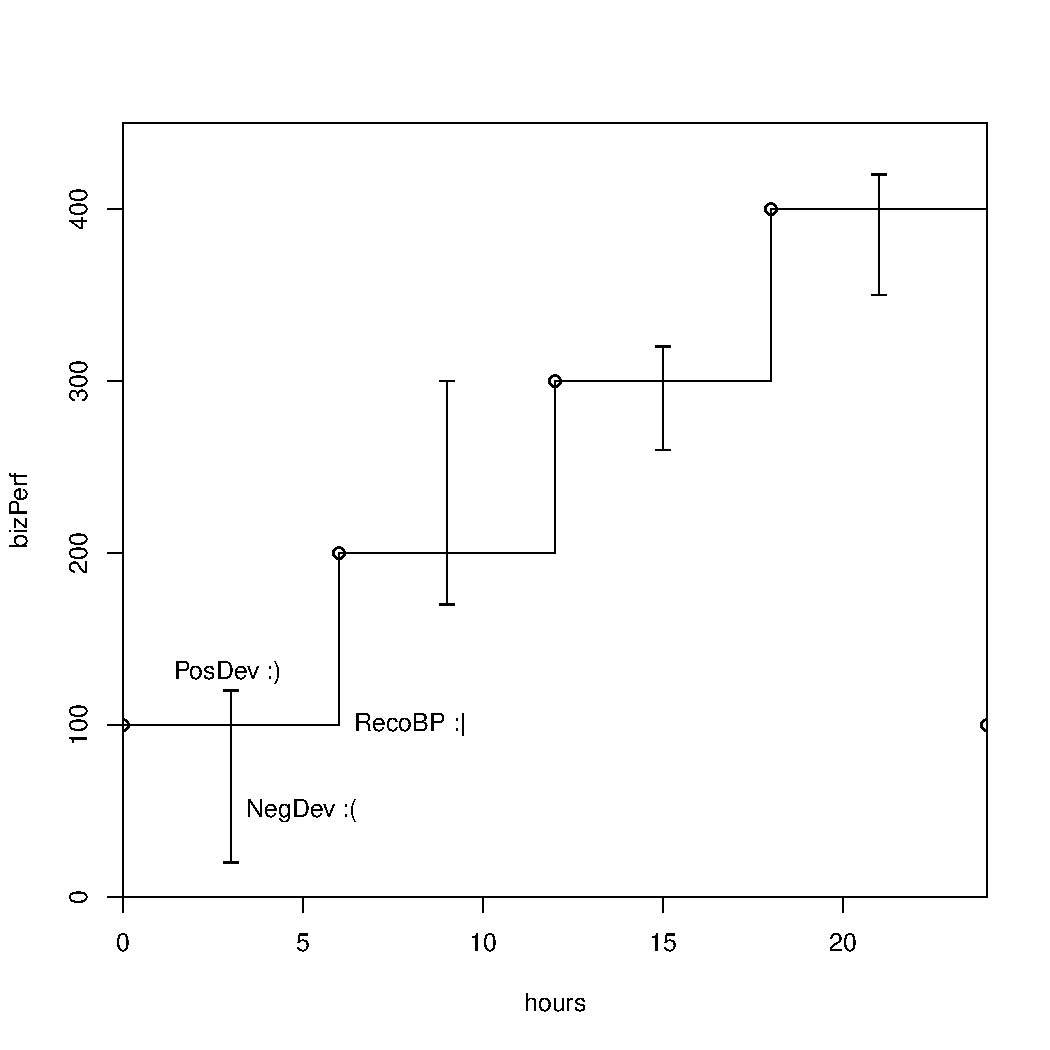
\includegraphics[width=0.99\linewidth]{generated/SFA-candles.pdf}
\caption{Service Flexibility Agreement representation}
\label{fig:SFA}
\end{figure}

\begin{listing}[h]
\begin{minted} [frame=single, linenos]{yaml}
SFA:
  - Time: 00:00 to 05:59
    RecoBP: 100 Hz
    PosDev: 20 Hz/H
    NegDev: 80 Hz/H
  - Time: 06:00 to 11:59
    RecoBP: 200 Hz
    PosDev: 100 Hz/H
    NegDev: 25 Hz/H

WorkingModes:
  - WMName: WM1
    actuator: 'cf scale myApp -i 3'
    defaultPower: '300 W'
    maxBusinessPerf: '100 Hz'
  - WMName: WM2
    actuator: 'cf scale myApp -i 5'
    defaultPower: '500 W'
    maxBusinessPerf: '150 Hz'
\end{minted}
\caption{SFA example}
\label{lst:SFA}
\end{listing}

As shown in listing~\ref{lst:SFA} and also represented graphically in figure~\ref{fig:SFA}, for each time frame of a day the SFA defines a recommended business performance (RecoBP, in red in the figure). 
The business performance is one of the KPIs of the application.
For example, for a Web server it is the number of pages served per minutes, for a video transcoding service it will be how many videos can be transcoded per minutes.

We then define a concept called "Happy points", noted "H".
This is an abstraction of the end-user satisfaction.
An application having zero Happy points means that the end user is reasonably satisfied.
An application being allocated exactly the number of resources corresponding to the RecoBP collects 0 Happy points.
This situation corresponds to the traditional SLA threshold.
The positive and negative deviations (PosDev and NegDev) declared in the SFA are then the way that each application "reacts" to being given more or less resources than the RecoBP.
Indeed, some applications such as video transcoding can benefit from receiving temporarily more resources because they can process more videos and thus make their end user happier. 
This kind of application reacts linearly to the amount of resources it is allocated.
On the other hand, an application such as a web server typically have a "turning point" in their relation between performance and resources.
Indeed, giving them less that a certain level of resources (such as the number of front-end VMs) will start to augment the latency in delivering web pages, thus making the end-user unhappy.
On the contrary, giving them more than that level of resources will not have any perceptible impact on the end user, as the latency is already small.
This is represented by the vertical deviation bars in figure~\ref{fig:SFA}: the length of the bar represents the amount of Happy points that the application will win/lose when given more/less performance than the recoBP, respectively.
In this example, at 10 O’clock, if the PaaS framework allocates the resource corresponding to the recommended business performance of 200Hz, the application will collect 0 Happy points.
If the application gets 300Hz, it will get 1H, and one more Happy point for each 100Hz above that.
Conversely, if it gets less than the recommended 200Hz, it will loose Happy point at the rate of one happy point per 25Hz.

We further define the various Working Modes (WM) of an application.
A WM corresponds to a set of resources allocated by the PaaS to an application.
We associate to each WM its typical power consumption and the maximum business performance it can offer.
In practice, a WM corresponds to a number of VMs or Linux Containers, each running instances of the application.
Using the SFA, it is now possible to compute the number of Happy points provided by each WM for each time slot.

